\section{Auswertung}
\label{sec:Auswertung}
Jegliche Fehlerrechnung wurde mit der python-Bibliothek uncertainties [3] absolviert.
Trotz dessen sind die Formeln für die Unsicherheiten in den jeweiligen Abschnitten angege-
ben. Allgemeine Rechnungen wurden mit der python-Bibliothek numpy [4] automatisiert.
Die graphischen Unterstützungen wurden mit Hilfe der python-Bibliothek matplotlib [2]
erstellt.
\subsection{Bestimmung der Strömungsgeschwindigkeit der Dopplerflüssgkeit}
Mit Hilfe der Gleichung $REFERENZ$ lässt sich die Strömungsgeschwindigkeit der Dopplerflüssgkeit bestimmen.
Zu den verschiedenen Rohrdurchmessern ($D_\text{dick} = \SI{16}{\milli\metre}$, $D_\text{mittel} = \SI{10}{\milli\metre}$,
$D_\text{klein} = \SI{7}{\milli\metre}$) sind die zu den Umdrehungen gemessenen Frequenzverschiebungen $\symup{\Delta} \nu$,
und die daraus errechneten Strömungsgeschwindigkeiten  in den Tabellen \ref{tab:big}, \ref{tab:middle} und \ref{tab:tiny} aufgetragen.

\begin{table}
    \centering
    \caption{Gemessene Frequenzverschiebungen
            und die daraus errechneten Strömungsgeschwindigkeiten ($D_\text{dick} = \SI{16}{\milli\metre}$)}
    \label{tab:big}
    \begin{tabular}{S[table-format=4.0]
                    S[table-format=2.0] S[table-format=1.3] 
                    S[table-format=3.0] S[table-format=2.3] 
                    S[table-format=3.0] S[table-format=2.3]}
        \toprule
        &
        \multicolumn{2}{c}{$\theta = \ang{15;;}$} &
        \multicolumn{2}{c}{$\theta = \ang{30;;}$} & 
        \multicolumn{2}{c}{$\theta = \ang{60;;}$} \\
        \cmidrule(lr){2-3} \cmidrule(lr){4-5} \cmidrule(lr){6-7}
        {$\text{rpm}$}&
        {$\symup{\Delta} \nu \mathbin{/} \si{\hertz}$} & {$v \mathbin{/} \si{\milli\meter\second\tothe{-1}}$} & 
        {$\symup{\Delta} \nu \mathbin{/} \si{\hertz}$} & {$v \mathbin{/} \si{\milli\meter\second\tothe{-1}}$} &
        {$\symup{\Delta} \nu \mathbin{/} \si{\hertz}$} & {$v \mathbin{/} \si{\milli\meter\second\tothe{-1}}$} \\
        \midrule
        5400 & 49 & 4.205 & 73  &  6.265 & 110 & 9.439 \\
        6200 & 61 & 5.235 & 98  &  8.410 & 146 & 12.529\\
        7000 & 73 & 6.265 & 116 & 9.955  & 183 & 15.704\\
        7800 & 85 & 7.295 & 122 & 10.470 & 208 & 17.849\\
        8400 & 98 & 8.411 & 159 & 13.645 & 250 & 21.453\\
    \end{tabular}
\end{table}
\begin{table}
    \centering
    \caption{Gemessene Frequenzverschiebungen
            und die daraus errechneten Strömungsgeschwindigkeiten ($D_\text{mittel} = \SI{10}{\milli\metre}$)}
    \label{tab:middle}
    \begin{tabular}{S[table-format=4.0]
                    S[table-format=3.0] S[table-format=2.3] 
                    S[table-format=3.0] S[table-format=2.3] 
                    S[table-format=3.0] S[table-format=3.3]}
        \toprule
        &
        \multicolumn{2}{c}{$\theta = \ang{15;;}$} &
        \multicolumn{2}{c}{$\theta = \ang{30;;}$} & 
        \multicolumn{2}{c}{$\theta = \ang{60;;}$} \\
        \cmidrule(lr){2-3} \cmidrule(lr){4-5} \cmidrule(lr){6-7}
        {$\text{rpm}$}&
        {$\symup{\Delta} \nu \mathbin{/} \si{\hertz}$} & {$v \mathbin{/} \si{\milli\meter\second\tothe{-1}}$} & 
        {$\symup{\Delta} \nu \mathbin{/} \si{\hertz}$} & {$v \mathbin{/} \si{\milli\meter\second\tothe{-1}}$} &
        {$\symup{\Delta} \nu \mathbin{/} \si{\hertz}$} & {$v \mathbin{/} \si{\milli\meter\second\tothe{-1}}$} \\
        \midrule
        5400 & 98  & 8.411 &  159 &  13.645 &  317 &  27.202 \\
        6200 & 122 & 10.471 &  208 & 17.851 &  354 &  30.377 \\
        7000 & 140 & 12.016 &  256 & 21.970 &  476 &  40.846 \\
        7800 & 171 & 14.676 &  330 & 28.321 &  610 &  52.345 \\
        8400 & 195 & 16.736 &  366 & 31.410 &  700 &  60.068 \\
    \end{tabular}
\end{table}
\begin{table}
    \centering
    \caption{Gemessene Frequenzverschiebungen
            und die daraus errechneten Strömungsgeschwindigkeiten ($D_\text{klein} = \SI{7}{\milli\metre}$)}
    \label{tab:tiny}
    \begin{tabular}{S[table-format=4.0]
                    S[table-format=3.0] S[table-format=2.3] 
                    S[table-format=3.0] S[table-format=2.3] 
                    S[table-format=4.0] S[table-format=3.3]}
        \toprule
        &
        \multicolumn{2}{c}{$\theta = \ang{15;;}$} &
        \multicolumn{2}{c}{$\theta = \ang{30;;}$} & 
        \multicolumn{2}{c}{$\theta = \ang{60;;}$} \\
        \cmidrule(lr){2-3} \cmidrule(lr){4-5} \cmidrule(lr){6-7}
        {$\text{rpm}$}&
        {$\symup{\Delta} \nu \mathbin{/} \si{\hertz}$} & {$v \mathbin{/} \si{\milli\meter\second\tothe{-1}}$} & 
        {$\symup{\Delta} \nu \mathbin{/} \si{\hertz}$} & {$v \mathbin{/} \si{\milli\meter\second\tothe{-1}}$} &
        {$\symup{\Delta} \nu \mathbin{/} \si{\hertz}$} & {$v \mathbin{/} \si{\milli\meter\second\tothe{-1}}$} \\
        \midrule
        5400 & 171 & 14.676 & 300 & 25.746 & 627 & 53.804  \\
        6200 & 220 & 18.882 & 427 & 36.645 & 720 & 61.785  \\
        7000 & 262 & 22.486 & 500 & 42.910 & 848 & 72.769  \\
        7800 & 317 & 27.207 & 635 & 54.496 & 1100& 94.393  \\
        8400 & 366 & 31.412 & 745 & 63.936 & 1324& 113.615  \\
    \end{tabular}
\end{table}
\begin{figure}
    \centering
    \caption(Quotient gegen die Strömungsgeschwindigkeit des dicken Rohrs)
    \label{fig:big}
    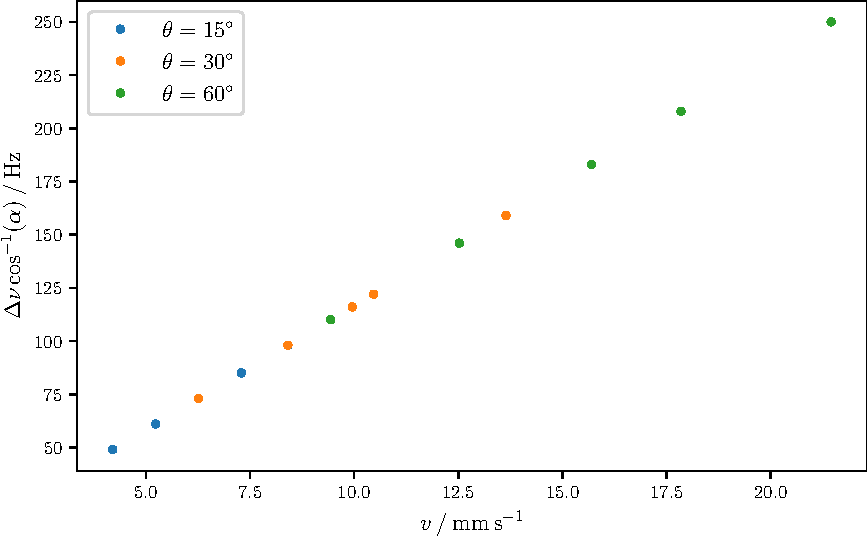
\includegraphics{build/big.pdf}
\end{figure}
\begin{figure}
    \centering
    \caption(Quotient gegen die Strömungsgeschwindigkeit des mittleren Rohrs)
    \label{fig:middle}
    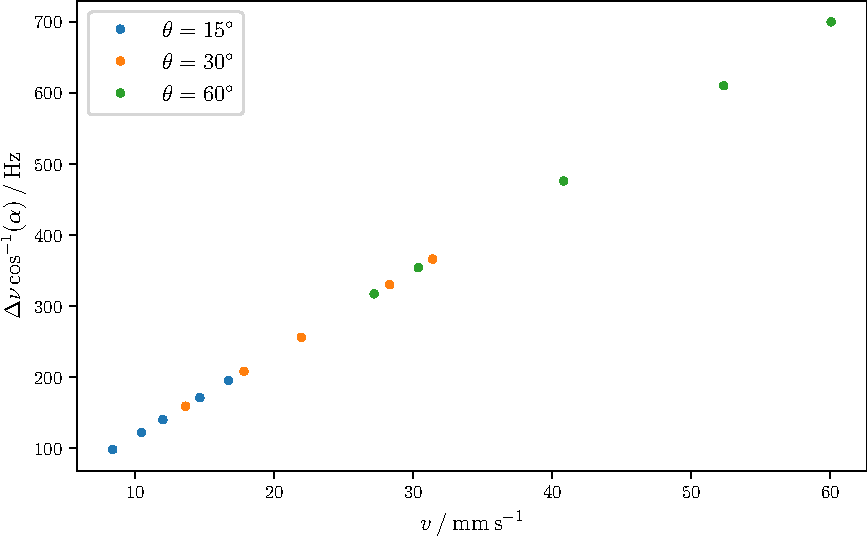
\includegraphics{build/middle.pdf}
\end{figure}
\begin{figure}
    \centering
    \caption(Quotient gegen die Strömungsgeschwindigkeit des dünnen Rohrs)
    \label{fig:tiny}
    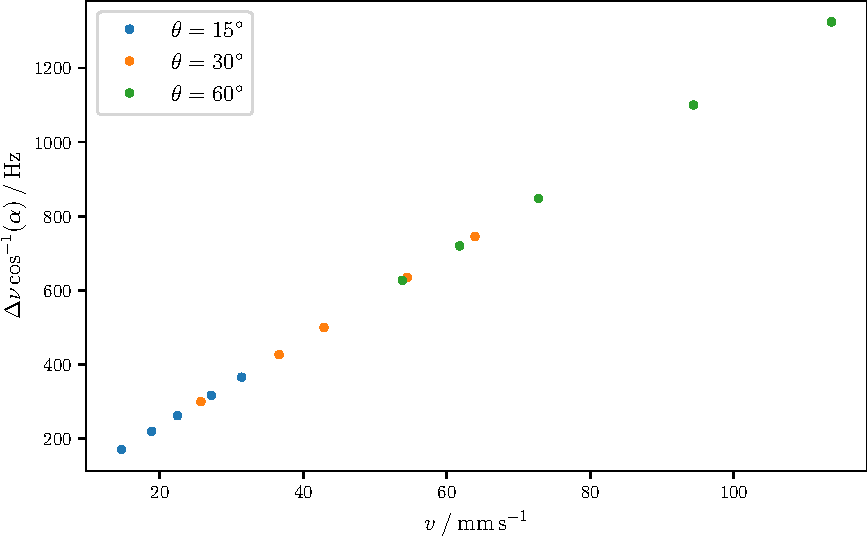
\includegraphics{build/tiny.pdf}
\end{figure}